\documentclass[a4paper, 12pt]{article}
\usepackage[utf8]{inputenc}
\usepackage[spanish]{babel}
\usepackage{url, hyperref}
\usepackage[table]{xcolor}
\usepackage{listings, xcolor}
\usepackage{adjustbox, subcaption}

\definecolor{codegreen}{rgb}{0,0.6,0}
\definecolor{codegray}{rgb}{0.5,0.5,0.5}
\definecolor{codepurple}{rgb}{0.58,0,0.82}
\definecolor{backcolour}{rgb}{0.95,0.95,0.92}

\lstdefinestyle{mystyle}{
    backgroundcolor=\color{backcolour},   
    commentstyle=\color{codegreen},
    keywordstyle=\color{magenta},
    numberstyle=\tiny\color{codegray},
    stringstyle=\color{codepurple},
    basicstyle=\ttfamily\footnotesize,
    breakatwhitespace=false,         
    breaklines=true,                 
    captionpos=b,                    
    keepspaces=true,                 
    numbers=left,                    
    numbersep=5pt,                  
    showspaces=false,                
    showstringspaces=false,
    showtabs=false,                  
    tabsize=2
}
\lstset{style=mystyle, language=Python}
\setlength{\parindent}{0pt}
\setlength{\parskip}{12pt}

\title{\vspace{-3cm}Tarea 7: Ladrón ambicioso (Knapsack) con GA}
\author{
    Universidad Autónoma de San Luis Potosí\\ 
    Facultad de Ingeniería - Ing. en Sistemas Inteligentes\\ 
    \textbf{Materia:} Cómputo Bioinspirado \\
    \textbf{Prof:} Dr. Cesar Augusto Puente Montejano  \\
    \textbf{Autor:} Angel de Jesús Maldonado Juárez
}
\date{\textbf{Fecha de entrega:} jueves 27 de octubre de 2022}

\begin{document}
\maketitle

\begin{center}
    \rule{\textwidth}{0.5pt}
    \begin{abstract}
        \noindent En la naturaleza existen muchos procesos que pueden ser utilizados como una fuente de soluciones comprobadas, la evolución de los seres vivos y la selección natural son procesos comprobados para solucionar el problema de la \emph{adaptación}. Los \emph{algoritmos genéticos} (GA), utilizan estos procesos naturales para simular la evolución y selección de individuos artificiales cuyo propósito es explorar su espacio para encontrar la solución más óptima a un problema. En este reporte se muestra la implementación y configuración del algoritmo genético en Python, utilizando la librería \emph{geneticalgoritm2}, para encontrar la maximización al problema de combinatoria \emph{Knapsack}.
    \end{abstract}
    \rule{\textwidth}{0.5pt}
\end{center}

\section{Algoritmos Genéticos}
La idea principal de los algoritmos genéticos es generar \emph{individuos artificiales} (soluciones) que sean sometidos a los mismos procesos naturales de \emph{selección}, \emph{mutación}, y \emph{adaptación} en un \emph{entorno} o \emph{espacio}, también es artificial, que representa un problema que se desee resolver. Este espacio en el que las entidades (soluciones) \emph{existen}, engloba las distintas posibilidades que los individuos pueden explorar, y al momento de probar la supervivencia de la población en el espacio del problema existirá una \emph{función de evaluación} que indica, numéricamente, qué tan óptimo es la genética de cada individuo de la población para encontrar una solución (\emph{fitness}). Posteriormente, se hará una selección de individuos con base en el valor \emph{fitness} que estos recibieron, aquellos que fueron seleccionados se reproducirán entre sí utilizando algún \emph{operador genético} para generar nuevos candidatos para encontrar la solución al problema, los cuales además de tener una combinación de las características de los individuos seleccionados, también tienen características únicas gracias a la \emph{mutación}.

\section{Python + librería \emph{geneticalgorithm2}}
Para este reporte se utiliza el framework de \emph{Python} con \emph{Anaconda} y la librería \emph{geneticalgorithm2}, la cual es una extensión de su versión original \emph{geneticalgorithm}, en donde implementa más parámetros configurables de visualización y para el desempeño del mismo algoritmo. Tiene a la librería \emph{NumPy} como única dependencia, e implementa varios operadores de cruzamiento, mutación, y selección, además soporta enteros, booleanos, y números reales (continuos y discretos) como tipos de variables. Entre otras funciones añadidas a la versión desactualizada son el algoritmo \emph{studEA} y las \emph{revoluciones}.

\section{Problema Knapsack utilizando GA}
El planteamiento del problema Knapsack (o mochila infinita) es el siguiente: Un ladrón llega a robar una casa. Para su buena suerte, encuentra un salón lleno de objetos sumamente valiosos. Para su mala suerte, solo lleva una pequeña mochila que puede soportar cuando mucho 10 kilogramos de peso. Por lo tanto, debe decidir cuáles objetos puede cargar, tratando de llevarse la mayor ganancia posible. Entre los que encontró están los siguientes:

\begin{table}[!ht]
    \begin{adjustbox}{width=\textwidth}
        \begin{tabular}{|c|c|c|c|c|c|c|c|}
            \hline
                  & Bolsa de centenarios & Billetes de \$1000 & Joyero grande & Joyero pequeño & Estampillas & Obra de arte & Pisapapeles de oro \\
            \hline
            Valor & \$750,000            & \$500,000          & \$2,750,000   & \$950,000      & \$1,850,000 & \$3,250,000  & \$3,950,000        \\
            \hline
            Peso  & 2.5kg                & 1kg                & 6kg           & 2.5kg          & 1.5kg       & 3kg          & 5kg                \\
            \hline
        \end{tabular}
    \end{adjustbox}
\end{table}

\subsection{Representación binaria de Knapsack}
Para poder plantear una solución al problema Knapsack utilizando el algoritmo genético. Primeramente se deben de representar las posibles selecciones de los objetos como un genotipo, esto puede ser utilizando un arreglo/lista en el/la que cada posición $i$ indica con un $1$ si se toma el objeto, y con un $0$ si no se toma, en la siguiente tabla (arreglo) se muestra una posible combinación de objetos seleccionados: Bolsa de centenarios, Joyero grande, y el Pisapapeles de oro:

\begin{table}[!ht]
    \centering
    \begin{tabular}{|c|c|c|c|c|c|c|}
        \hline
        $X_0$ & $X_1$ & $X_2$ & $X_3$ & $X_4$ & $X_5$ & $X_6$ \\
        \hline
        1     & 0     & 1     & 0     & 0     & 0     & 1     \\
        \hline
    \end{tabular}
\end{table}

\subsection{Funciones del problema}
Tomando en cuenta el planteamiento inicial, se tiene que: dados $n$ objetos de peso $w_i$ y valor $v_i$ (con $i=1...n$), se deben seleccionar cuáles objetos se meten a la mochila, la cual soporta un peso máximo $P$, de manera que se \textbf{maximice} el valor total de los objetos introducidos.

Por lo tanto, la función a maximizar es la sumatoria ($Z$) del valor ($v_j$) de los objetos ($x_j$) elegidos ($x=1$):

\begin{equation}\label{eq:1}
    Z = \sum_{j = 1}^{n}v_jx_j
\end{equation}

Tomando en cuenta que la función de restricción es que la suma ($R$) de los pesos ($p_j$) de los objetos ($x_j$) elegidos ($x=1$) no deben ser mayores a la capacidad de la mochila ($P=10$):

\begin{equation}\label{eq:2}
    R = \sum_{j = 1}^{n}p_jx_j \longrightarrow  R \leq 10
\end{equation}

\subsection{Implementación}
Antes de poner en marcha el algoritmo genético, se debe realizar la implementación de la \emph{función fitness} (función de aptitud) que evalúa la viabilidad de un genotipo o individuo para solucionar el problema. Para la implementación de esta función se requiere definir la estructura de los objetos y un conjunto en donde puedan inicializarse los 7 objetos del problema. El siguiente script en Python (archivo \lstinline{knapsack.py}) muestra la definición de la clase \lstinline{Object}, la cual tiene como propiedades el nombre del objeto \lstinline{n}, su peso \lstinline{w}, y su valor \lstinline{v}:

\begin{lstlisting}
class Object:
    def __init__(self, n: str, w: float, v: float) -> None:
        self.n = n
        self.w = w
        self.v = v
\end{lstlisting}

Después, se crea el arreglo \lstinline{objects} donde se inicializan los 7 objetos del problema utilizando la clase \lstinline{Object}:

\begin{lstlisting}
objects = [
    Object(n='Centenarios', w=2.5, v=750000.00),
    Object(n='Billetes de 1k', w=1.0, v=500000.00),
    Object(n='Joyero gde', w=6.0, v=2750000.00),
    Object(n='Joyero ch', w=2.5, v=950000.00),
    Object(n='Estampillas', w=1.5, v=1850000.00),
    Object(n='Obra de arte', w=3.0, v=3250000.00),
    Object(n='Pisapapeles', w=5.0, v=3950000.00),
]
\end{lstlisting}

Posteriormente, se crean las variables \lstinline{max_w} (para establecer el peso máximo que la mochila soporta) y \lstinline{objects_count} (que indica la cantidad de objetos del problema):

\begin{lstlisting}
max_w = 10.0
objects_count = len(objects)
\end{lstlisting}

Para la implementación de la función de aptitud (\emph{fitness}) se requiere la importación de la librería \emph{List} (\lstinline{from typing import List}) para especificar que el parámetro de la función es una lista con los objetos que son o no seleccionados, y se indica que el valor de retorno es un número flotante (\lstinline{->float}). La primera línea de código representa la función de maximización del valor de los objetos \lstinline{vSum}, la segunda es la sumatoria de los pesos de los objetos \lstinline{wSum}, y la tercera línea representa la restricción del problema donde indica que la función \lstinline{knapsack} retornará el valor de \lstinline{vSum} (sumatoria del valor de los objetos) si el peso acumulado de los objetos no sobrepasa el límite de la mochila (\lstinline{if wSum < max_w}), de lo contrario retorna \lstinline{0} y el algoritmo genético descartará el genotipo/individuo de la población:

\begin{lstlisting}
def knapsack(X: List) -> float:
    vSum = sum([X[index] * objects[index].v for index in range(objects_count)])
    wSum = sum([X[index] * objects[index].w for index in range(objects_count)])
    return vSum if wSum < max_w else 0
\end{lstlisting}

Las importaciones para el archivo principal \lstinline{ga.py} son las siguientes:

\begin{lstlisting}
import knapsack as ks
import numpy as np
import matplotlib.pyplot as plt
# for creating and running optimization model
from geneticalgorithm2 import geneticalgorithm2 as ga
# classes for comfortable parameters setting and getting
from geneticalgorithm2 import *
\end{lstlisting}

Debido a que la librería \emph{geneticalgorithm2} realiza minimización por defecto en el archivo principal se crea una función \lstinline{fitness()} que retorna el valor de la función \lstinline{ks.knapsack()} multiplicado por -1, para que el algoritmo funcione correctamente, y al final simplemente el valor absoluto de los resultados que se muestren serán los correctos:

\begin{lstlisting}
def fitness(X): return -ks.knapsack(X)
\end{lstlisting}

Posteriormente, se definen los límites de los 7 genes como una tupla de falso y verdadero (\lstinline{(False, True)}) en la variable \lstinline{varBound}:

\begin{lstlisting}
varBound = [(False, True)] * int(ks.objects_count)
\end{lstlisting}

Los parámetros para la ejecución del algoritmo se crean utilizando el constructor \lstinline{AlgorithmParams()} y se asignan a la variable \lstinline{params}, únicamente se modifica el tamaño de la población \lstinline{population_size} para empezar con una población pequeña ($7$):

\begin{lstlisting}
params = AlgorithmParams(
    max_num_iteration=None,
    population_size=7,
    mutation_probability=0.1,
    mutation_discrete_probability=None,
    elit_ratio=0.01,
    crossover_type='uniform',
    mutation_type='uniform_by_center',
    mutation_discrete_type='uniform_discrete',
    selection_type='roulette',
    max_iteration_without_improv=None
)
\end{lstlisting}

Los demás parámetros se dejan con sus valores por defecto, sin embargo, en las demás ejecuciones se modifican algunos de ellos para mejorar el resultado.

Se crea el modelo del algoritmo genético asignando la función de aptitud \lstinline{fitness}, la dimensión \lstinline{ks.objects_count}, el tipo de variable \lstinline{'bool'}, los límites de las variables \lstinline{varBound}, los parámetros del algoritmo \lstinline{params}, y se establece un tiempo máximo de ejecución (\lstinline{function_timeout}) de 60 segundos:

\begin{lstlisting}
model = ga(
    function=fitness,
    dimension=ks.objects_count,
    variable_type='bool',
    variable_boundaries=varBound,
    function_timeout=60,
    algorithm_parameters=params
)
\end{lstlisting}

Finalmente, se ejecuta el modelo asignando el resultado de este a la variable \lstinline{result}, y estableciendo que no genere una gráfica (\lstinline{no_plot=True}):

\begin{lstlisting}
result = model.run(no_plot=True)
\end{lstlisting}

Los resultados que el algoritmo mostrará en la terminal tendrán signo negativo debido a que por defecto el algoritmo minimiza, así que simplemente se considerarán sus valores absolutos. Y para mostrar una gráfica adecuada a la maximización se utiliza la variable \lstinline{model} para obtener el valor absoluto del historial de la función de aptitud:

\begin{lstlisting}
report = np.abs(np.array(model.report))
plt.plot(report)
plt.xlabel('Iteration')
plt.ylabel('Knapsack Value')
plt.title('Genetic Algorithm for Knapsack')
plt.show()
\end{lstlisting}

\subsection{Resultados}
La siguiente tabla muestra los valores para las distintas configuraciones y resultados del algoritmo GA resolviendo la función de maximización $Z$ (\ref{eq:1}) con la restricción $R$ (\ref{eq:2}) utilizando la librería \emph{geneticalgorithm2} de Python:

\begin{table}[!ht]
    \begin{adjustbox}{width=\textwidth}
        \begin{tabular}{|c|c|c|c|c|c|c|c|c|}
            \rowcolor{yellow}
            \hline
            max\_it & $pop\_size$ & $mut\_prob$ & $elit\_rat$ & $par\_port$ & $crossover$ & Tiempo      & $Z(x)$    \\
            \hline
            $50$    & $7$         & $0.1$       & $0.01$      & $0.3$       & uniform     & $0.0172sec$ & $6800000$ \\
            \hline
            $52$    & $7$         & $0.1$       & $0.01$      & $0.3$       & uniform     & $0.022sec$  & $9050000$ \\
            \hline
        \end{tabular}
    \end{adjustbox}
\end{table}

Debido a que el espacio a explorar no es tan grande, el algoritmo es bastante eficiente para encontrar la solución simplemente con una población de la misma cantidad de objetos que hay ($7$). Incluso algunas corridas con el parámetro \lstinline{max_num_iteration} establecido en $50$ dieron el mismo resultado óptimo ($9050000$), pero a partir de \lstinline{max_num_iteration} en $52$ la mayoría de corridas ya dan el resultado óptimo. Las siguientes gráficas muestran la comparativa entre el peor resultado obtenido contra el mejor, seguido de las poblaciones para la peor corrida y la mejor corrida que el algoritmo generó son las siguientes:

\begin{figure}[!ht]
    \centering
    \begin{subfigure}[b]{0.48\textwidth}
        \centering
        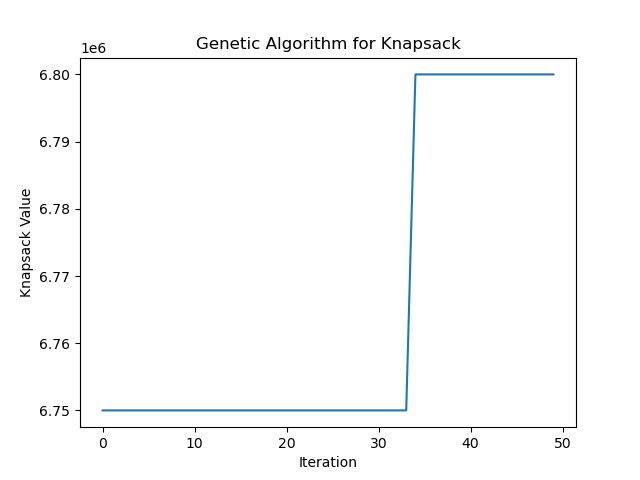
\includegraphics[width=\textwidth]{img/corrida_1.png}
        \caption{Peor corrida}
        \label{subfig:corrida1}
    \end{subfigure}
    \hfill
    \begin{subfigure}[b]{0.48\textwidth}
        \centering
        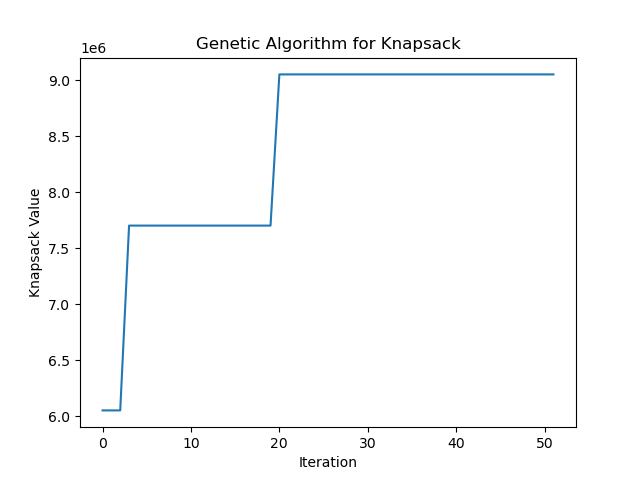
\includegraphics[width=\textwidth]{img/corrida_2.png}
        \caption{Mejor corrida}
        \label{subfig:corrida2}
    \end{subfigure}
    \caption{Peor corrida vs. mejor corrida (Knapsack con GA)}
\end{figure}

\begin{figure}[!ht]
    \centering
    \begin{subfigure}[b]{0.48\textwidth}
        \centering
        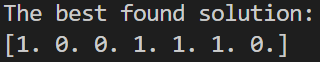
\includegraphics[width=\textwidth]{img/corrida_1pob.png}
        \caption{Mejor individuo peor corrida}
        \label{subfig:corrida1pob}
    \end{subfigure}
    \hfill
    \begin{subfigure}[b]{0.48\textwidth}
        \centering
        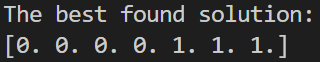
\includegraphics[width=\textwidth]{img/corrida_2pob.png}
        \caption{Mejor individuo mejor corrida}
        \label{subfig:corrida2pob}
    \end{subfigure}
    \caption{Individuo peor corrida vs. mejor corrida (Knapsack con GA)}
\end{figure}

\section{Conclusiones}
El algoritmo genético es una buena alternativa para encontrar soluciones a problemas de complejidad muy alta, o que la cantidad de posibilidades aumente de forma exponencial. Y a pesar de que se dependa en gran medida del factor aleatorio que el algoritmo tiene para la generación de nuevos individuos en la población, y que estos sean quienes encuentren una mejor solución, es mucho más rápido que cualquier otro algoritmo. Además, identificar las características y parámetros clave de un problema para crear un genotipo resulta sencillo una vez que se identifican las funciones de maximización (o minimización), y aplicar las restricciones del problema utilizando un lenguaje de programación tan flexible como Python también resulta sencillo de implementar.

\bibliographystyle{unsrt}
\bibliography{refs}
\nocite{*}
\end{document}